% Chapter 3: Reinforcement Learning for Parameter Optimization
% IEEE-style textbook chapter


The optimization of synthetic data generator parameters presents a challenging black-box optimization problem characterized by expensive function evaluations, complex parameter interactions, and noisy gradients. This chapter provides a comprehensive treatment of reinforcement learning and related optimization algorithms suitable for discovering optimal parameter configurations that maximize downstream object detection performance. We examine the theoretical foundations, algorithmic details, and practical considerations for deploying these methods in resource-constrained settings where each evaluation requires training a complete neural network.

\section{Algorithm Selection for Expensive Black-Box Optimization}
\label{sec:algorithm_selection}

The selection of an appropriate optimization algorithm for synthetic data generator parameter tuning requires careful consideration of the problem's unique characteristics. Unlike typical reinforcement learning scenarios where millions of environment interactions are feasible, our setting imposes severe sample budget constraints. Each evaluation of a parameter configuration necessitates generating synthetic training data, training a YOLO object detection model, and evaluating performance on real-world test images. This process typically requires several hours of computation, limiting practical budgets to hundreds or at most a few thousand evaluations.

\subsection{Limitations of Traditional Reinforcement Learning}
\label{subsec:rl_limitations}

Traditional reinforcement learning algorithms such as Proximal Policy Optimization, Trust Region Policy Optimization, and Advantage Actor-Critic methods were designed for scenarios involving millions of environment interactions. These algorithms rely on statistical averaging over large numbers of samples to reduce variance in gradient estimates and ensure stable policy improvement. The sample complexity of policy gradient methods scales poorly with the dimensionality of the action space and the stochasticity of the environment, making them ill-suited for expensive black-box optimization.

Policy gradient methods estimate the gradient of expected return with respect to policy parameters through Monte Carlo sampling of trajectories. The variance of these gradient estimates is inherently high, particularly in early stages of training when the policy explores broadly. Techniques such as baseline subtraction and advantage normalization reduce but do not eliminate this variance, necessitating large batch sizes for stable learning. In the context of generator parameter optimization, where each trajectory sample requires hours of computation, collecting sufficient samples for reliable gradient estimation becomes prohibitively expensive.

Off-policy algorithms such as Soft Actor-Critic and Twin Delayed Deep Deterministic Policy Gradient offer improved sample efficiency through experience replay, enabling multiple gradient updates from each collected transition. However, even these methods typically require tens of thousands of environment interactions to converge to good policies. The fundamental limitation stems from the need to learn both the value function and the policy from scratch, without leveraging any prior knowledge about the structure of the optimization landscape.

The credit assignment problem presents additional challenges in the generator optimization setting. The reward signal, derived from object detection metrics such as mean average precision, reflects the cumulative effect of all parameter choices but provides limited information about which specific parameters contributed positively or negatively to performance. Traditional reinforcement learning algorithms address credit assignment through temporal difference learning over long trajectories, but in our single-step optimization setting, this mechanism offers no benefit.

\subsection{The Case for Bayesian Optimization}
\label{subsec:bayesian_case}

Bayesian optimization provides a principled framework for sequential decision-making under uncertainty that is particularly well-suited to expensive black-box optimization. Rather than learning a policy through trial and error, Bayesian optimization maintains a probabilistic surrogate model of the objective function and uses this model to guide exploration toward promising regions of the parameter space. This approach explicitly reasons about uncertainty, enabling intelligent allocation of the limited evaluation budget.

The surrogate model, typically a Gaussian process, provides not only predictions of the objective function value at unobserved points but also uncertainty estimates that reflect how confident the model is in these predictions. High uncertainty indicates regions where additional evaluations would provide substantial information gain, while low uncertainty with high predicted values indicates regions likely to contain the optimum. Acquisition functions such as Expected Improvement, Upper Confidence Bound, and Knowledge Gradient formalize this exploration-exploitation tradeoff, selecting query points that maximize expected utility given the current model.

Gaussian process models offer several advantages for generator parameter optimization. They require no gradient information from the objective function, handling the non-differentiable composition of data generation, network training, and evaluation seamlessly. They provide calibrated uncertainty estimates that accurately reflect epistemic uncertainty about the objective landscape. They naturally handle noisy observations through the inclusion of a noise variance term in the likelihood. Perhaps most importantly, they are data-efficient, achieving good optimization performance with orders of magnitude fewer evaluations than gradient-based methods.

The Tree-Parzen Estimator provides an alternative probabilistic modeling approach that scales more gracefully to high-dimensional parameter spaces. Rather than modeling the objective function directly, Tree-Parzen Estimators model the conditional probability of parameter configurations given that they produce good or bad objective values. This formulation avoids the cubic scaling of Gaussian process inference with the number of observations, enabling application to larger budgets and higher-dimensional spaces.

Figure~\ref{fig:exploration_exploitation} illustrates the fundamental exploration-exploitation tradeoff in Bayesian optimization, showing how acquisition functions balance the predicted objective value (exploitation) against uncertainty in predictions (exploration).

\begin{figure}[htbp]
\centering
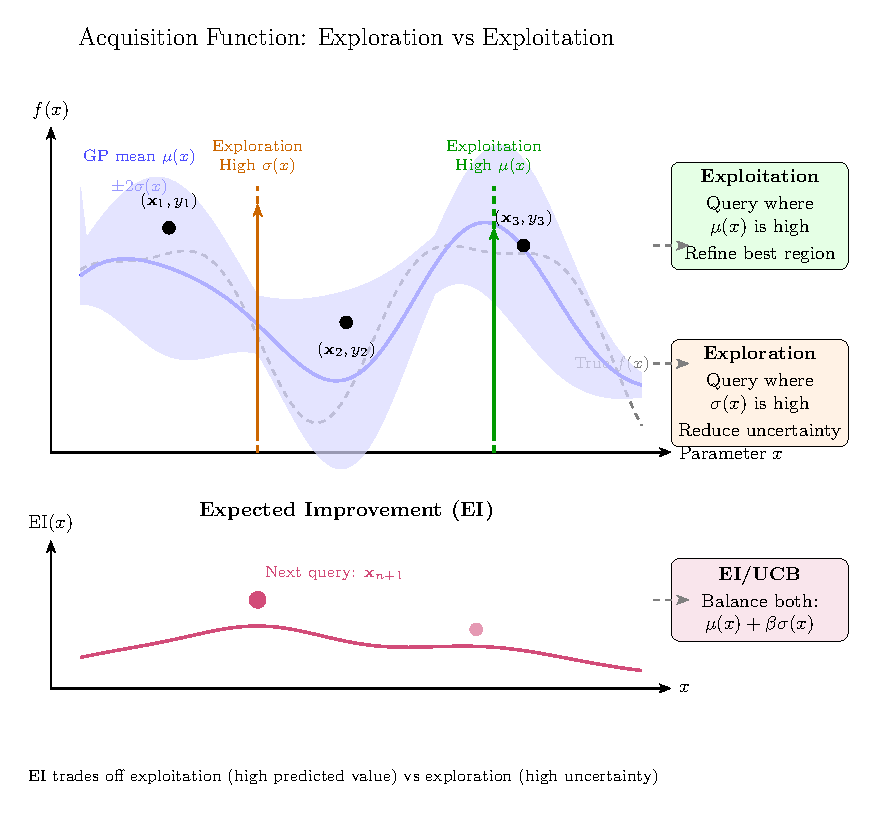
\includegraphics[width=0.95\textwidth]{figures/ch03_fig3_exploration_exploitation.pdf}
\caption{Exploration versus exploitation in Bayesian optimization. The top panel shows a Gaussian process surrogate model with mean prediction (solid line) and uncertainty band (shaded region). Observed data points reduce uncertainty locally. Exploitation favors regions with high predicted values, while exploration targets regions with high uncertainty. The bottom panel shows the Expected Improvement acquisition function, which combines both objectives to select the next query point. The acquisition function peaks in regions that offer either high predicted performance or substantial uncertainty reduction.}
\label{fig:exploration_exploitation}
\end{figure}

\subsection{Comparative Analysis of Optimization Algorithms}
\label{subsec:algorithm_comparison}

The selection of an optimization algorithm depends critically on the problem characteristics, including dimensionality, budget constraints, presence of categorical parameters, and computational resources available for surrogate model fitting. Table~\ref{tab:algorithm_comparison} provides a comprehensive comparison of leading algorithms across these dimensions.

\begin{table}[htbp]
\centering
\caption{Comparison of Optimization Algorithms for Expensive Black-Box Problems}
\label{tab:algorithm_comparison}
\renewcommand{\arraystretch}{1.3}
\begin{tabular}{|p{2.2cm}|p{1.8cm}|p{1.5cm}|p{2.0cm}|p{2.2cm}|p{2.5cm}|}
\hline
\textbf{Algorithm} & \textbf{Sample Efficiency} & \textbf{Max Dims} & \textbf{Handles Categorical} & \textbf{Parallelization} & \textbf{Best Use Case} \\
\hline
GP-BO (EI/UCB) & Very High & 10--20 & Limited & Batch acquisition & Low-dim continuous \\
\hline
TPE & High & 50--100 & Native & Independent sampling & Mixed spaces \\
\hline
SMAC & High & 100+ & Native & Racing & Algorithm config \\
\hline
TuRBO & Very High & 20--50 & Limited & Trust regions & High-dim continuous \\
\hline
BOHB & High & 50+ & Native & Parallel brackets & Multi-fidelity \\
\hline
CMA-ES & Moderate & 100+ & No & Population & Continuous only \\
\hline
PBT & Moderate & 20--50 & Limited & Highly parallel & Schedule learning \\
\hline
PPO & Low & Unlimited & Yes & Parallel envs & Dense rewards \\
\hline
SAC & Low--Moderate & Unlimited & Limited & Limited & Continuous control \\
\hline
\end{tabular}
\end{table}

Gaussian Process Bayesian Optimization with Expected Improvement or Upper Confidence Bound acquisition functions represents the gold standard for sample efficiency in low-dimensional continuous optimization. The cubic scaling of exact Gaussian process inference limits applicability to approximately twenty dimensions and a few thousand observations, though sparse approximations and local models extend this range. For generator optimization problems with fewer than twenty continuous parameters, this approach offers the best expected performance per evaluation.

The Tree-Parzen Estimator relaxes the dimensionality constraints of Gaussian processes while maintaining strong sample efficiency. By modeling the density of configurations separately for those above and below a performance threshold, TPE avoids the computational burden of full joint modeling. The kernel density estimation approach handles mixed continuous and categorical parameters naturally, making TPE particularly suitable for generator optimization where parameters may include discrete choices such as augmentation types or continuous values such as noise levels.

Sequential Model-based Algorithm Configuration extends Bayesian optimization with random forests as the surrogate model, offering superior handling of categorical and conditional parameters. The random forest surrogate scales linearly with the number of observations and handles high cardinality categorical variables without explicit encoding. SMAC's racing mechanism provides additional efficiency by early-stopping clearly inferior configurations, making it well-suited for scenarios where partial evaluations provide informative signals.

Trust Region Bayesian Optimization addresses the curse of dimensionality through a local modeling approach that maintains multiple trust regions around promising configurations. Rather than building a single global surrogate model, TuRBO fits local Gaussian process models within each trust region and adapts region sizes based on optimization progress. Successful evaluations expand the trust region to enable broader exploration, while failures contract it to focus on exploitation. This approach achieves state-of-the-art performance on optimization benchmarks with up to fifty dimensions.

Covariance Matrix Adaptation Evolution Strategy provides a gradient-free optimization method based on evolving a multivariate normal sampling distribution. CMA-ES adapts both the mean and covariance matrix of the distribution based on the ranking of sampled solutions, enabling automatic discovery of appropriate step sizes and parameter correlations. While less sample-efficient than Bayesian methods for very expensive objectives, CMA-ES offers robust performance across a wide range of problem types and scales well to high dimensions. The algorithm is particularly effective when parallel evaluation of population members is possible.


\section{BOHB: Bayesian Optimization with Hyperband}
\label{sec:bohb}

Bayesian Optimization with Hyperband represents a principled integration of Bayesian optimization's sample efficiency with Hyperband's multi-fidelity scheduling. This combination addresses a fundamental limitation of standard Bayesian optimization: the assumption that all function evaluations have equal cost. In practice, many optimization problems admit cheap approximations to the full objective, such as training with fewer epochs or evaluating on a subset of the data. BOHB exploits this structure to dramatically accelerate optimization by allocating resources adaptively based on early performance signals.

\subsection{Theoretical Foundations}
\label{subsec:bohb_theory}

The theoretical justification for BOHB rests on the observation that performance rankings of configurations often stabilize before full evaluation completes. If a configuration performs poorly with a small computational budget, it is unlikely to become optimal with additional resources. This observation motivates early stopping of unpromising configurations to redirect resources toward more promising alternatives. Hyperband formalizes this intuition through successive halving, progressively eliminating the worst-performing fraction of configurations at each stage.

The integration with Bayesian optimization addresses Hyperband's primary weakness: random configuration sampling. While Hyperband efficiently allocates resources among sampled configurations, the quality of the initial sample critically determines final performance. By replacing random sampling with Tree-Parzen Estimator-guided sampling, BOHB combines the adaptive resource allocation of Hyperband with the informed exploration of Bayesian optimization.

The theoretical analysis of BOHB establishes regret bounds that interpolate between pure Bayesian optimization and pure Hyperband depending on the correlation structure between cheap and expensive evaluations. When cheap evaluations are highly predictive of expensive ones, BOHB achieves near-optimal sample complexity with respect to the cheap fidelity while maintaining guarantees with respect to the true objective. This formal analysis provides guidance on when multi-fidelity optimization offers substantial benefits versus when standard Bayesian optimization suffices.

\subsection{Tree-Parzen Estimator Sampler}
\label{subsec:tpe}

The Tree-Parzen Estimator provides the probabilistic model underlying BOHB's configuration sampling. Unlike Gaussian process-based Bayesian optimization, which models the objective function directly as $p(y | \mathbf{x})$, TPE models the inverse relationship $p(\mathbf{x} | y)$ by separately estimating densities for good and bad configurations. This reformulation offers computational advantages and natural handling of complex parameter spaces.

The algorithm partitions observed configurations into two groups based on a quantile threshold $\gamma$, typically set to 0.15 or 0.25. Configurations with objective values in the top $\gamma$ quantile form the good set $\mathcal{D}_\ell$, while the remainder form the bad set $\mathcal{D}_g$. Kernel density estimation constructs probability density functions $\ell(\mathbf{x})$ and $g(\mathbf{x})$ over the parameter space for each group. The acquisition function then evaluates configurations based on the density ratio, preferring regions where good configurations are dense relative to bad ones.

For continuous parameters, TPE employs truncated Gaussian kernels centered on observed values, with bandwidth adapted to the local density of observations. The truncation ensures that sampled configurations respect parameter bounds. For categorical parameters, TPE uses a weighted mixture model that places probability mass on observed categories proportionally to their frequency in the good set, with a small uniform component for exploration.

The Expected Improvement acquisition function under the TPE model takes a particularly simple form. Rather than requiring numerical integration as in Gaussian process-based methods, the TPE formulation yields the closed-form expression:

\begin{equation}
\text{EI}(\mathbf{x}) \propto \frac{\gamma + (1-\gamma) \cdot g(\mathbf{x})/\ell(\mathbf{x})}{1}
\end{equation}

Maximizing Expected Improvement thus reduces to maximizing $\ell(\mathbf{x})/g(\mathbf{x})$, which is achieved by sampling candidates from $\ell(\mathbf{x})$ and evaluating the ratio. This procedure is computationally efficient and scales gracefully to high dimensions through the factorized density model.

\subsection{Integration with Successive Halving}
\label{subsec:successive_halving}

Successive halving provides the resource allocation mechanism within BOHB. Given a set of configurations and a budget constraint, successive halving evaluates all configurations at the minimum fidelity, eliminates the worst-performing fraction, and repeats with increased fidelity for survivors until only one configuration remains or the maximum fidelity is reached. This geometric progression of resources ensures that promising configurations receive exponentially more evaluation time than unpromising ones.

The key parameters governing successive halving are the minimum and maximum fidelities $r_{\min}$ and $r_{\max}$, the reduction factor $\eta$ (typically 3), and the bracket structure determining how many configurations to sample initially. Hyperband addresses the exploration-exploitation tradeoff in choosing the initial sample size by running multiple brackets in parallel, ranging from aggressive exploration with many configurations at low fidelity to conservative exploitation with few configurations at high fidelity.

BOHB modifies standard Hyperband by replacing random sampling with TPE-guided sampling within each bracket. As evaluations complete across brackets, the TPE model incorporates results from all fidelities, enabling transfer of information between cheap and expensive evaluations. This shared modeling allows insights gained from low-fidelity evaluations to immediately influence sampling at high fidelities, accelerating convergence.

Algorithm~\ref{alg:bohb} presents the complete BOHB procedure, highlighting the interaction between Hyperband's bracket structure and TPE's probabilistic sampling.

\begin{algorithm}[htbp]
\caption{Bayesian Optimization with Hyperband (BOHB)}
\label{alg:bohb}
\begin{algorithmic}[1]
\Require Maximum budget $R$, minimum budget $r$, reduction factor $\eta$, quantile $\gamma$
\Ensure Best configuration $\mathbf{x}^*$ and corresponding objective value $y^*$
\State $s_{\max} \gets \lfloor \log_\eta(R/r) \rfloor$
\State $B \gets (s_{\max} + 1) \cdot R$ \Comment{Total budget per Hyperband round}
\State Initialize observation history $\mathcal{H} \gets \emptyset$
\State Initialize TPE models $\ell(\cdot), g(\cdot)$
\For{each Hyperband iteration}
    \For{$s \in \{s_{\max}, s_{\max}-1, \ldots, 0\}$} \Comment{Bracket loop}
        \State $n \gets \lceil \frac{B}{R} \cdot \frac{\eta^s}{s+1} \rceil$ \Comment{Initial configurations}
        \State $r_0 \gets R \cdot \eta^{-s}$ \Comment{Initial budget per config}
        \If{$|\mathcal{H}| < n_{\text{init}}$}
            \State Sample $n$ configurations uniformly at random: $\mathcal{T} \gets \{\mathbf{x}_1, \ldots, \mathbf{x}_n\}$
        \Else
            \State Fit TPE models $\ell(\cdot), g(\cdot)$ from $\mathcal{H}$ using quantile $\gamma$
            \State Sample $n$ configurations from $\ell(\cdot)$ maximizing $\ell(\mathbf{x})/g(\mathbf{x})$: $\mathcal{T} \gets \{\mathbf{x}_1, \ldots, \mathbf{x}_n\}$
        \EndIf
        \For{$i \in \{0, 1, \ldots, s\}$} \Comment{Successive halving rounds}
            \State $n_i \gets \lfloor n \cdot \eta^{-i} \rfloor$
            \State $r_i \gets r_0 \cdot \eta^i$
            \State Evaluate $\mathcal{T}$ with budget $r_i$: $\{y_{\mathbf{x}} : \mathbf{x} \in \mathcal{T}\}$
            \State Update history: $\mathcal{H} \gets \mathcal{H} \cup \{(\mathbf{x}, y_{\mathbf{x}}, r_i) : \mathbf{x} \in \mathcal{T}\}$
            \State Retain top $\lfloor n_i / \eta \rfloor$ configurations: $\mathcal{T} \gets \text{top}_k(\mathcal{T}, \lfloor n_i / \eta \rfloor)$
        \EndFor
    \EndFor
\EndFor
\State \Return $\mathbf{x}^* \gets \arg\min_{\mathbf{x} \in \mathcal{H}_{r=R}} y_{\mathbf{x}}$
\end{algorithmic}
\end{algorithm}

Figure~\ref{fig:bohb_diagram} provides a visual representation of the BOHB algorithm, illustrating how the Tree-Parzen Estimator guides configuration sampling while successive halving progressively eliminates underperforming configurations across multiple fidelity levels.

\begin{figure}[htbp]
\centering
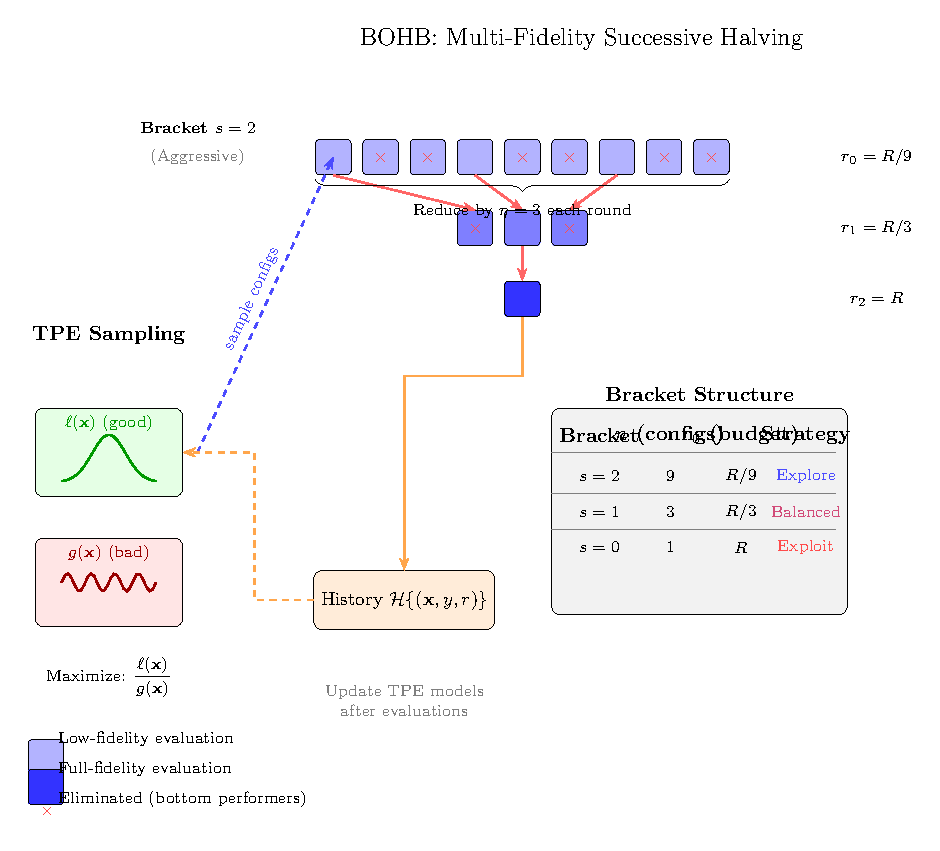
\includegraphics[width=0.95\textwidth]{figures/ch03_fig2_bohb.pdf}
\caption{BOHB algorithm overview showing the integration of TPE-guided sampling with successive halving. The bracket structure (shown for $s=2$) demonstrates how configurations are progressively evaluated at increasing fidelity levels, with the worst performers eliminated at each round. The TPE sampler models the density of good configurations $\ell(\mathbf{x})$ versus bad configurations $g(\mathbf{x})$, maximizing their ratio to propose promising new configurations. The history $\mathcal{H}$ accumulates results from all fidelity levels to continuously improve the surrogate model.}
\label{fig:bohb_diagram}
\end{figure}

\subsection{Theoretical Guarantees and Convergence}
\label{subsec:bohb_guarantees}

The theoretical analysis of BOHB provides convergence guarantees under reasonable assumptions on the relationship between low-fidelity and high-fidelity evaluations. Let $f_r(\mathbf{x})$ denote the objective at fidelity $r$ and $f_R(\mathbf{x})$ denote the objective at maximum fidelity. The key assumption is that the ranking induced by $f_r$ over configurations is partially preserved in $f_R$, formalized through bounds on the probability that the true optimum is eliminated at low fidelity.

Under these assumptions, BOHB achieves a regret bound that depends on the effective dimensionality of the parameter space and the correlation between fidelities. When correlations are strong, BOHB's regret approaches that of an oracle with access to the full fidelity evaluation at cost equal to the minimum fidelity. When correlations are weak, BOHB gracefully degrades to standard Hyperband performance with the additional overhead of TPE model fitting.

The practical implication of these guarantees is that BOHB provides robustness across a range of problem characteristics. When multi-fidelity structure is exploitable, BOHB automatically discovers and leverages this structure. When such structure is absent, BOHB remains competitive with single-fidelity methods through the quality of its configuration sampling.


\section{Population-Based Training}
\label{sec:pbt}

Population-Based Training provides an alternative paradigm for hyperparameter optimization that combines the parallelism of random search with the adaptivity of sequential optimization. Rather than optimizing hyperparameters before training begins, PBT optimizes them during training by maintaining a population of agents that share information through periodic exploitation and exploration operations. This online approach naturally discovers hyperparameter schedules rather than fixed values, offering potential advantages for problems where optimal hyperparameters change over the course of optimization.

\subsection{Algorithm Description}
\label{subsec:pbt_algorithm}

Population-Based Training maintains a population of $N$ agents, each with its own model parameters $\theta_i$ and hyperparameters $h_i$. Agents train independently for a fixed interval, after which they evaluate performance on a validation metric. Low-performing agents exploit high-performing ones by copying their model parameters and hyperparameters, then explore by perturbing the copied hyperparameters. This process repeats throughout training, enabling the population to collectively discover effective hyperparameter schedules.

The exploitation step implements a form of truncation selection. Each agent compares its performance to the population and, if in the bottom fraction (typically 20\%), selects a replacement from the top fraction. The selection may be uniform among top performers or weighted by performance. After exploitation, the agent's model parameters are replaced with those of the selected parent, providing a warm start for continued training.

The exploration step perturbs hyperparameters of agents that have just exploited. Perturbations may be multiplicative (scaling by factors such as 0.8 or 1.2), additive (adding noise from a specified distribution), or resampling from prior distributions. The perturbation scheme should be matched to the hyperparameter types and scales, with multiplicative perturbations typically preferred for learning rates and regularization strengths.

Algorithm~\ref{alg:pbt} provides a detailed specification of the Population-Based Training procedure.

\begin{algorithm}[htbp]
\caption{Population-Based Training (PBT)}
\label{alg:pbt}
\begin{algorithmic}[1]
\Require Population size $N$, exploitation fraction $\rho$, perturbation factors $\mathcal{P}$
\Ensure Trained models $\{\theta_i\}_{i=1}^N$ with discovered schedules
\State Initialize population $\{(\theta_i, h_i)\}_{i=1}^N$ with random hyperparameters
\State Initialize step counters $\{t_i \gets 0\}_{i=1}^N$
\While{not converged}
    \For{each agent $i \in \{1, \ldots, N\}$ in parallel}
        \State Train for $\Delta t$ steps: $\theta_i \gets \text{Train}(\theta_i, h_i, \Delta t)$
        \State $t_i \gets t_i + \Delta t$
        \State Evaluate performance: $p_i \gets \text{Evaluate}(\theta_i)$
    \EndFor
    \State Compute performance ranking of population
    \For{each agent $i$ with $p_i$ in bottom $\rho$ fraction}
        \State \textbf{Exploit:} Select parent $j$ from top $\rho$ fraction
        \State Copy parameters: $\theta_i \gets \theta_j$
        \State Copy hyperparameters: $h_i \gets h_j$
        \State \textbf{Explore:} Perturb hyperparameters
        \For{each hyperparameter $h_i^{(k)}$}
            \State Sample perturbation $\delta \sim \mathcal{P}$
            \State Apply: $h_i^{(k)} \gets h_i^{(k)} \cdot \delta$ \Comment{or additive}
        \EndFor
    \EndFor
\EndWhile
\State \Return $\{\theta_i\}_{i=1}^N$
\end{algorithmic}
\end{algorithm}

\subsection{Discovering Parameter Schedules}
\label{subsec:pbt_schedules}

A distinguishing feature of Population-Based Training is its ability to discover hyperparameter schedules without explicit parameterization. Because hyperparameters are adapted during training, the sequence of values encountered by agents that eventually achieve high performance constitutes an implicitly learned schedule. Post-hoc analysis of these trajectories reveals patterns that may generalize to future training runs.

The schedule discovery property is particularly valuable for learning rate optimization, where the optimal value typically decreases over training. Traditional approaches require specifying a schedule a priori, such as exponential decay or cosine annealing, with parameters that must themselves be tuned. PBT discovers effective schedules automatically, often finding non-monotonic patterns that outperform standard schedules.

Beyond learning rate, PBT has discovered effective schedules for regularization strength, data augmentation intensity, and exploration parameters in reinforcement learning. In each case, the optimal trajectory depends on the current state of training in ways that are difficult to specify analytically but emerge naturally from the population dynamics.

\subsection{Extensions: GPBT and IPBT}
\label{subsec:pbt_extensions}

Guided Population-Based Training addresses a limitation of standard PBT: the random exploration step may require many generations to discover beneficial hyperparameter changes. GPBT replaces random perturbation with surrogate model-guided search, using a Gaussian process or random forest to model the relationship between hyperparameters and performance given the current training state. This guidance accelerates discovery of effective hyperparameters while maintaining the online adaptation property.

Importance-Weighted Population-Based Training modifies the exploitation mechanism to account for the relative difficulty of different training stages. Rather than uniform exploitation throughout training, IPBT adjusts the exploitation frequency and intensity based on the marginal value of hyperparameter adaptation at each stage. Early in training, when the landscape changes rapidly, frequent exploitation is valuable. Later, when the landscape stabilizes, exploitation overhead may outweigh benefits.

These extensions share the goal of improving sample efficiency while preserving PBT's core advantages. GPBT reduces the number of generations required to discover effective schedules by replacing random exploration with informed search. IPBT reduces computational overhead by adapting exploitation frequency to the current training regime. Both approaches have demonstrated improvements over standard PBT on benchmark tasks.

\subsection{When to Prefer PBT over BOHB}
\label{subsec:pbt_vs_bohb}

The choice between Population-Based Training and BOHB depends on several problem characteristics. PBT offers advantages when hyperparameters should vary during optimization, when massively parallel evaluation is available, and when the optimization horizon is long enough for population dynamics to operate effectively. BOHB offers advantages when hyperparameters are fixed during optimization, when sequential evaluation is acceptable, and when the budget is too limited for population-based approaches.

For generator parameter optimization, the appropriate choice depends on whether parameters should remain fixed throughout YOLO training or adapt as training progresses. If the generator runs once at the beginning of each training run, producing a fixed dataset, then BOHB's sample efficiency makes it the preferred choice. If the generator could be integrated into the training loop, producing new samples adaptively, then PBT's schedule discovery becomes relevant.

Computational considerations also influence the choice. PBT requires maintaining $N$ parallel training runs throughout optimization, with $N$ typically ranging from 10 to 100. For expensive training procedures, this requirement may exceed available resources. BOHB's sequential nature with optional parallelization over brackets provides more flexibility in resource allocation.


\section{Continuous Control RL Methods}
\label{sec:continuous_control}

While Bayesian optimization methods offer superior sample efficiency for expensive black-box optimization, reinforcement learning algorithms designed for continuous control remain relevant in specific scenarios. When the optimization horizon extends to allow thousands of evaluations, when the action space has special structure that policies can exploit, or when transfer learning from related tasks is possible, modern actor-critic algorithms may become competitive. This section provides detailed treatment of Soft Actor-Critic and Twin Delayed DDPG, the leading algorithms for continuous control.

\subsection{Soft Actor-Critic}
\label{subsec:sac}

Soft Actor-Critic represents the state of the art in off-policy reinforcement learning for continuous action spaces. The algorithm combines three key innovations: an actor-critic architecture with separate policy and value function approximators, off-policy learning through experience replay, and maximum entropy regularization that encourages exploration and improves robustness.

The maximum entropy framework augments the standard reinforcement learning objective with an entropy bonus, yielding the maximum entropy objective:

\begin{equation}
J(\pi) = \sum_{t=0}^{T} \mathbb{E}_{(\mathbf{s}_t, \mathbf{a}_t) \sim \rho_\pi} \left[ r(\mathbf{s}_t, \mathbf{a}_t) + \alpha \mathcal{H}(\pi(\cdot | \mathbf{s}_t)) \right]
\end{equation}

where $\mathcal{H}(\pi(\cdot | \mathbf{s})) = -\mathbb{E}_{\mathbf{a} \sim \pi}[\log \pi(\mathbf{a} | \mathbf{s})]$ is the entropy of the policy at state $\mathbf{s}$, and $\alpha$ is a temperature parameter controlling the relative importance of entropy versus reward. Higher entropy policies spread probability mass across actions, encouraging exploration and preventing premature convergence to deterministic solutions.

The practical benefits of maximum entropy regularization extend beyond exploration. Policies with higher entropy are more robust to perturbations in the environment dynamics, as they maintain probability mass on alternative actions. This robustness property is particularly valuable in transfer settings, where policies trained in simulation must generalize to real-world conditions that differ from training.

Soft Actor-Critic employs two soft Q-functions to address overestimation bias, taking the minimum of their predictions when computing target values. The soft Q-function is defined as:

\begin{equation}
Q^\pi(\mathbf{s}_t, \mathbf{a}_t) = r(\mathbf{s}_t, \mathbf{a}_t) + \gamma \mathbb{E}_{\mathbf{s}_{t+1} \sim p} \left[ V^\pi(\mathbf{s}_{t+1}) \right]
\end{equation}

where the soft value function incorporates the entropy bonus:

\begin{equation}
V^\pi(\mathbf{s}) = \mathbb{E}_{\mathbf{a} \sim \pi} \left[ Q^\pi(\mathbf{s}, \mathbf{a}) - \alpha \log \pi(\mathbf{a} | \mathbf{s}) \right]
\end{equation}

The policy is represented as a Gaussian with state-dependent mean and variance, parameterized by a neural network. Actions are sampled using the reparameterization trick, enabling gradient-based optimization of the policy through the Q-function:

\begin{equation}
\mathbf{a}_t = \mu_\phi(\mathbf{s}_t) + \sigma_\phi(\mathbf{s}_t) \odot \epsilon, \quad \epsilon \sim \mathcal{N}(0, I)
\end{equation}

The temperature parameter $\alpha$ may be fixed or learned automatically. Automatic temperature adjustment optimizes $\alpha$ to maintain a target entropy level, adapting the exploration-exploitation tradeoff to the current policy's behavior. This automatic tuning eliminates a sensitive hyperparameter and improves performance across diverse tasks.

\begin{algorithm}[htbp]
\caption{Soft Actor-Critic (SAC)}
\label{alg:sac}
\begin{algorithmic}[1]
\Require Learning rates $\lambda_Q, \lambda_\pi, \lambda_\alpha$, target entropy $\bar{\mathcal{H}}$, discount $\gamma$, soft update rate $\tau$
\Ensure Trained policy $\pi_\phi$
\State Initialize Q-networks $Q_{\theta_1}, Q_{\theta_2}$ and target networks $Q_{\bar{\theta}_1}, Q_{\bar{\theta}_2}$
\State Initialize policy network $\pi_\phi$ and temperature $\alpha$
\State Initialize replay buffer $\mathcal{D} \gets \emptyset$
\For{each iteration}
    \For{each environment step}
        \State Sample action: $\mathbf{a}_t \sim \pi_\phi(\cdot | \mathbf{s}_t)$
        \State Execute action, observe $\mathbf{s}_{t+1}, r_t$
        \State Store transition: $\mathcal{D} \gets \mathcal{D} \cup \{(\mathbf{s}_t, \mathbf{a}_t, r_t, \mathbf{s}_{t+1})\}$
    \EndFor
    \For{each gradient step}
        \State Sample minibatch $\mathcal{B} = \{(\mathbf{s}, \mathbf{a}, r, \mathbf{s}')\}$ from $\mathcal{D}$
        \State Sample next actions: $\tilde{\mathbf{a}}' \sim \pi_\phi(\cdot | \mathbf{s}')$
        \State Compute target Q-value:
        \State \quad $y = r + \gamma \left( \min_{j=1,2} Q_{\bar{\theta}_j}(\mathbf{s}', \tilde{\mathbf{a}}') - \alpha \log \pi_\phi(\tilde{\mathbf{a}}' | \mathbf{s}') \right)$
        \State Update Q-functions:
        \State \quad $\theta_i \gets \theta_i - \lambda_Q \nabla_{\theta_i} \frac{1}{|\mathcal{B}|} \sum_{(\mathbf{s},\mathbf{a},r,\mathbf{s}')} (Q_{\theta_i}(\mathbf{s}, \mathbf{a}) - y)^2$
        \State Sample actions for policy update: $\tilde{\mathbf{a}} \sim \pi_\phi(\cdot | \mathbf{s})$
        \State Update policy:
        \State \quad $\phi \gets \phi - \lambda_\pi \nabla_\phi \frac{1}{|\mathcal{B}|} \sum_\mathbf{s} \left( \alpha \log \pi_\phi(\tilde{\mathbf{a}} | \mathbf{s}) - \min_{j} Q_{\theta_j}(\mathbf{s}, \tilde{\mathbf{a}}) \right)$
        \State Update temperature:
        \State \quad $\alpha \gets \alpha - \lambda_\alpha \nabla_\alpha \frac{1}{|\mathcal{B}|} \sum_\mathbf{s} \left( -\alpha \log \pi_\phi(\tilde{\mathbf{a}} | \mathbf{s}) - \alpha \bar{\mathcal{H}} \right)$
        \State Soft update targets: $\bar{\theta}_i \gets \tau \theta_i + (1-\tau) \bar{\theta}_i$
    \EndFor
\EndFor
\State \Return $\pi_\phi$
\end{algorithmic}
\end{algorithm}

\subsection{Twin Delayed DDPG}
\label{subsec:td3}

Twin Delayed Deep Deterministic Policy Gradient builds on the DDPG algorithm by addressing three sources of instability: overestimation bias in the Q-function, high variance updates from stale critic estimates, and sensitivity to hyperparameters. The resulting algorithm achieves competitive performance with SAC while using a deterministic policy, avoiding the entropy computation and stochastic policy optimization of SAC.

The twin Q-functions of TD3 address overestimation through the clipped double Q-learning update. Target values are computed using the minimum of two Q-function predictions:

\begin{equation}
y = r + \gamma \min_{j=1,2} Q_{\bar{\theta}_j}(\mathbf{s}', \pi_{\bar{\phi}}(\mathbf{s}'))
\end{equation}

This pessimistic estimate counteracts the optimistic bias that arises from maximizing over noisy Q-value estimates.

Delayed policy updates reduce variance by updating the policy less frequently than the Q-functions, typically once per two Q-function updates. This allows the Q-functions to stabilize before influencing the policy, reducing the propagation of errors from critic to actor.

Target policy smoothing adds noise to target actions, regularizing the Q-function to be smooth with respect to actions:

\begin{equation}
\tilde{\mathbf{a}}' = \pi_{\bar{\phi}}(\mathbf{s}') + \epsilon, \quad \epsilon \sim \text{clip}(\mathcal{N}(0, \sigma), -c, c)
\end{equation}

This smoothing prevents the policy from exploiting narrow peaks in the Q-function landscape that may not correspond to genuinely high-value actions.

\subsection{Maximum Entropy Framework}
\label{subsec:max_entropy}

The maximum entropy framework provides theoretical grounding for the exploration bonuses used in SAC and related algorithms. By treating the reinforcement learning problem as inference in a probabilistic graphical model, maximum entropy methods derive principled objectives that balance reward maximization with maintaining uncertainty about the optimal solution.

The soft Bellman equation generalizes the standard Bellman equation to incorporate entropy:

\begin{equation}
Q^\pi(\mathbf{s}, \mathbf{a}) = r(\mathbf{s}, \mathbf{a}) + \gamma \mathbb{E}_{\mathbf{s}'} \left[ \mathbb{E}_{\mathbf{a}' \sim \pi} \left[ Q^\pi(\mathbf{s}', \mathbf{a}') - \alpha \log \pi(\mathbf{a}' | \mathbf{s}') \right] \right]
\end{equation}

The optimal policy under this framework takes the form of a Boltzmann distribution over the Q-function:

\begin{equation}
\pi^*(\mathbf{a} | \mathbf{s}) = \exp\left( \frac{1}{\alpha} \left( Q^*(\mathbf{s}, \mathbf{a}) - V^*(\mathbf{s}) \right) \right)
\end{equation}

This exponential policy form arises naturally from the variational characterization of the maximum entropy problem and connects reinforcement learning to probabilistic inference.

The benefits of maximum entropy extend to transfer and robustness. Policies with higher entropy assign non-negligible probability to suboptimal actions, enabling recovery when the environment differs from training. This property is particularly valuable for sim-to-real transfer, where simulation artifacts may have caused the policy to rely on details that do not hold in reality.

Figure~\ref{fig:policy_gradient} illustrates the flow of gradients through the policy network in actor-critic methods, highlighting the role of the reparameterization trick and entropy regularization.

\begin{figure}[htbp]
\centering
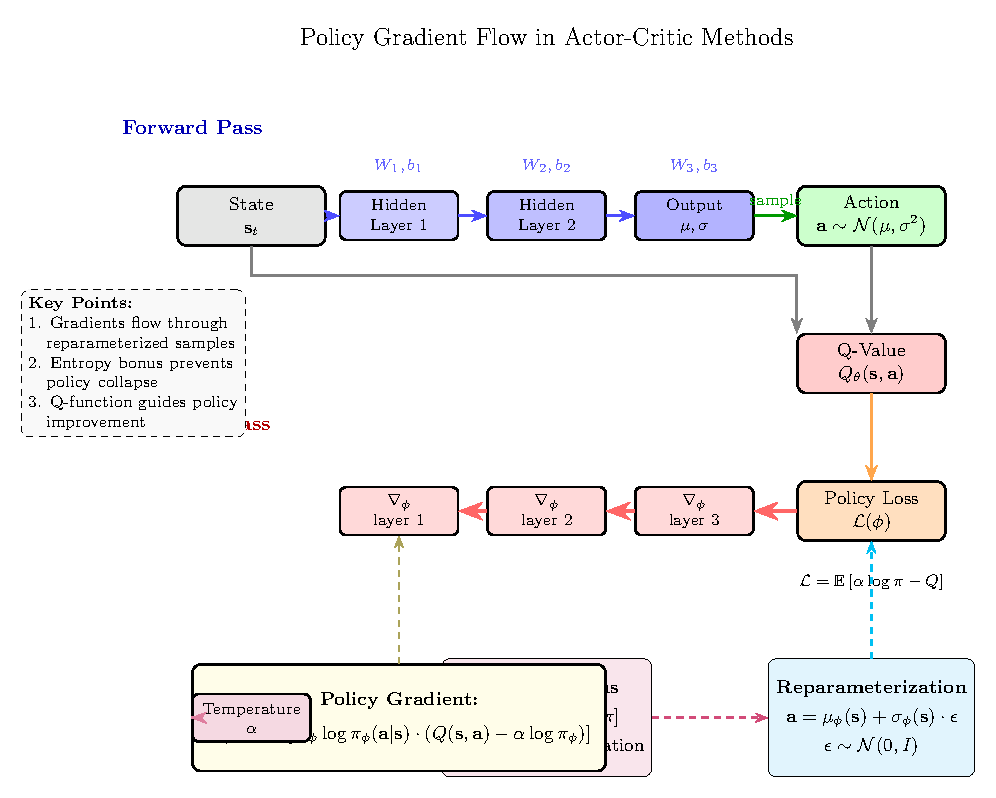
\includegraphics[width=0.95\textwidth]{figures/ch03_fig4_policy_gradient.pdf}
\caption{Policy gradient flow in actor-critic methods. The forward pass propagates state information through the policy network to produce action distributions, from which actions are sampled using the reparameterization trick. The Q-function evaluates state-action pairs to compute the policy loss. The backward pass propagates gradients through the reparameterized samples back to the policy parameters. The entropy bonus, controlled by temperature $\alpha$, encourages exploration by penalizing low-entropy policies. Key aspects include: (1) gradients flow through reparameterized samples enabling end-to-end optimization, (2) the entropy term prevents premature convergence to deterministic policies, and (3) the Q-function guides policy improvement toward high-value actions.}
\label{fig:policy_gradient}
\end{figure}

\subsection{Sample Efficiency Comparison}
\label{subsec:rl_sample_efficiency}

The sample efficiency of reinforcement learning algorithms varies substantially depending on problem characteristics and algorithmic details. Table~\ref{tab:rl_efficiency} summarizes typical sample requirements for achieving baseline performance across continuous control benchmarks.

\begin{table}[htbp]
\centering
\caption{Sample Efficiency of Continuous Control RL Algorithms}
\label{tab:rl_efficiency}
\renewcommand{\arraystretch}{1.3}
\begin{tabular}{|p{2.5cm}|p{2.0cm}|p{2.5cm}|p{2.0cm}|p{2.5cm}|}
\hline
\textbf{Algorithm} & \textbf{Samples to Baseline} & \textbf{Gradient Updates per Sample} & \textbf{Off-Policy} & \textbf{Continuous Actions} \\
\hline
PPO & 1--10M & 1 & No & Yes \\
\hline
TRPO & 1--10M & 1 & No & Yes \\
\hline
SAC & 100K--1M & 1--20 & Yes & Yes \\
\hline
TD3 & 100K--1M & 1 & Yes & Yes \\
\hline
DroQ-SAC & 10K--100K & 20 & Yes & Yes \\
\hline
REDQ & 10K--100K & 20 & Yes & Yes \\
\hline
\end{tabular}
\end{table}

Recent advances in sample-efficient reinforcement learning have reduced the gap between RL methods and Bayesian optimization. The Dropout Q-functions algorithm achieves strong performance with only tens of thousands of environment interactions through aggressive use of experience replay, performing twenty gradient updates per environment step. Similarly, Randomized Ensemble Double Q-learning maintains an ensemble of Q-functions to reduce overestimation, enabling data-efficient learning.

Despite these advances, the sample requirements of even the most efficient reinforcement learning algorithms exceed typical budgets for generator parameter optimization by one to two orders of magnitude. Reinforcement learning methods become competitive only when evaluation costs can be reduced through surrogate modeling or multi-fidelity approximation, or when prior knowledge can be transferred from related optimization tasks.


\section{State and Action Space Design}
\label{sec:state_action_design}

The design of state and action representations critically influences the performance of both reinforcement learning and Bayesian optimization methods. Effective representations compress the relevant information for decision-making while remaining tractable for function approximation or density modeling. This section examines design considerations for representing generator parameters as actions and encoding relevant state information.

\subsection{Representing Generator Parameters as Actions}
\label{subsec:parameter_actions}

Generator parameters form the natural action space for parameter optimization agents. Each configuration of the generator corresponds to a point in the action space, and the optimization objective is to find the action that maximizes downstream detection performance. The structure of this action space depends on the types and ranges of generator parameters.

Continuous parameters such as noise variance, object scale ranges, and lighting intensity map directly to bounded continuous action dimensions. The bounds should reflect physically meaningful or empirically determined limits on parameter values. Normalization of actions to a standard range, typically $[-1, 1]$ or $[0, 1]$, facilitates learning by ensuring that all dimensions contribute comparably to network activations.

The choice of parameterization affects optimization difficulty. For example, representing a scale range as (minimum, maximum) creates constraints that the minimum must not exceed the maximum. Alternative parameterizations such as (center, width) or (minimum, width) may simplify the feasible region, though they change the meaning of uniform sampling over the space.

\subsection{Continuous versus Discrete Parameter Handling}
\label{subsec:continuous_discrete}

Many generator configurations involve both continuous and discrete parameters. Discrete parameters include categorical choices such as augmentation types, texture categories, or background scenes, as well as integer parameters such as the number of objects per image. Handling mixed continuous-discrete spaces requires either specialized algorithms or careful encoding strategies.

One-hot encoding transforms categorical parameters into binary vectors, expanding the action space dimensionality but enabling application of continuous optimization methods. A categorical parameter with $k$ categories becomes $k$ binary dimensions with the constraint that exactly one is active. Relaxation approaches treat these dimensions as continuous probabilities, sampling from the resulting categorical distribution or taking the argmax for evaluation.

Ordinal parameters with natural ordering, such as discretized intensity levels, may be treated as continuous and rounded to the nearest valid value. This approach preserves gradient information through the rounding operation, enabling gradient-based optimization. However, rounding can create plateaus in the objective landscape where small parameter changes produce no change in the discrete value.

Tree-structured parameter spaces arise when some parameters are conditional on others. For example, the parameters of a specific augmentation are only relevant if that augmentation is enabled. Modeling these dependencies explicitly improves sample efficiency by avoiding evaluation of configurations with irrelevant parameters set to arbitrary values. The Tree-Parzen Estimator and SMAC handle conditional spaces natively, while standard Gaussian process models require explicit encoding.

\subsection{Hierarchical Action Spaces}
\label{subsec:hierarchical_actions}

Hierarchical action spaces decompose the full configuration into groups that can be optimized at different granularities or timescales. This decomposition reflects structure in the optimization problem, where some parameters may interact strongly within groups but weakly across groups. Exploiting this structure improves scalability to high-dimensional configuration spaces.

A two-level hierarchy might distinguish between coarse parameters that dramatically affect data distribution, such as object categories and scene types, and fine parameters that provide detailed control, such as exact placement distributions and noise levels. The outer level searches over coarse configurations while the inner level optimizes fine parameters conditional on the coarse choice. This decomposition reduces effective dimensionality at each level while preserving the ability to optimize the full space.

Temporal hierarchies adapt parameters at different frequencies during training. Slowly-varying parameters such as the overall difficulty of generated scenes might be adjusted every few epochs, while rapidly-varying parameters such as specific augmentation probabilities might change every batch. This temporal structure aligns with Population-Based Training's schedule discovery capability.

\subsection{State Representation}
\label{subsec:state_representation}

While pure black-box optimization treats each evaluation independently, incorporating state information can improve optimization efficiency by enabling transfer of knowledge across the optimization trajectory. Relevant state information includes the current parameter configuration, the history of previous evaluations, and summary statistics of the current training run.

The current parameter configuration provides context for value function learning in reinforcement learning approaches. Rather than learning a single optimal configuration, the value function can learn a landscape over configurations, enabling generalization and accelerating exploration. This state representation is implicit in Bayesian optimization through the surrogate model but requires explicit design in policy-based methods.

Historical performance metrics summarize the optimization trajectory, indicating which regions have been explored and how performance has evolved. Including this history enables policies to condition decisions on past experience, implementing forms of adaptive exploration. Encoding history efficiently requires compression, such as maintaining running statistics or using recurrent architectures.

Training dynamics metrics such as current loss, gradient norms, or validation performance provide real-time signals that may inform parameter adjustment before full evaluation completes. These signals enable early stopping of unpromising configurations or adaptive parameter adjustment during training, connecting to the multi-fidelity optimization framework.

Table~\ref{tab:action_space} summarizes typical action space dimensions for generator parameter optimization.

\begin{table}[htbp]
\centering
\caption{Action Space Dimensions for Generator Parameter Optimization}
\label{tab:action_space}
\renewcommand{\arraystretch}{1.3}
\begin{tabular}{|p{3.5cm}|p{2.0cm}|p{2.5cm}|p{4.0cm}|}
\hline
\textbf{Parameter Category} & \textbf{Type} & \textbf{Dimensions} & \textbf{Example Parameters} \\
\hline
Object placement & Continuous & 4--8 & Position range, scale range, rotation range \\
\hline
Lighting conditions & Continuous & 3--6 & Intensity, direction, color temperature \\
\hline
Scene composition & Mixed & 5--10 & Object count, clutter level, occlusion rate \\
\hline
Noise and artifacts & Continuous & 2--4 & Gaussian noise, motion blur, compression \\
\hline
Augmentation selection & Categorical & 10--20 & Flip, crop, color jitter probabilities \\
\hline
Domain parameters & Mixed & 5--15 & Background type, texture, weather conditions \\
\hline
\textbf{Total typical range} & Mixed & \textbf{30--60} & Full generator configuration \\
\hline
\end{tabular}
\end{table}


\section{Experience Replay and Sample Efficiency}
\label{sec:experience_replay}

Sample efficiency is paramount in expensive black-box optimization, where each evaluation may require hours of computation. This section examines techniques for maximizing the information extracted from each evaluation, including advanced experience replay strategies, transfer learning approaches, and surrogate model construction.

\subsection{Prioritized Experience Replay}
\label{subsec:per}

Prioritized Experience Replay improves sample efficiency by replaying transitions in proportion to their learning value rather than uniformly at random. Transitions with high temporal difference error indicate regions where the value function is poorly calibrated, suggesting that additional learning from these transitions would be beneficial. By focusing gradient updates on informative transitions, PER accelerates learning from limited data.

The priority of transition $i$ is defined based on its temporal difference error:

\begin{equation}
p_i = |\delta_i| + \epsilon
\end{equation}

where $\delta_i = r_i + \gamma V(\mathbf{s}'_i) - Q(\mathbf{s}_i, \mathbf{a}_i)$ is the TD error, and $\epsilon$ is a small constant ensuring non-zero probability for all transitions. The sampling probability follows a power law:

\begin{equation}
P(i) = \frac{p_i^\alpha}{\sum_k p_k^\alpha}
\end{equation}

where $\alpha$ controls the degree of prioritization, with $\alpha = 0$ recovering uniform sampling.

Non-uniform sampling introduces bias into gradient estimates, as transitions with high priority contribute disproportionately to learning. Importance sampling weights correct for this bias:

\begin{equation}
w_i = \left( \frac{1}{N \cdot P(i)} \right)^\beta
\end{equation}

where $\beta$ controls the degree of correction, typically annealed from a low initial value to 1 over training. Full correction ($\beta = 1$) eliminates bias at the cost of higher variance.

For generator parameter optimization, prioritized replay can be adapted to emphasize configurations with surprising performance, either much better or much worse than predicted by a surrogate model. This adaptation aligns the RL notion of TD error with the Bayesian optimization notion of information gain, bridging the two paradigms.

\subsection{Transfer Learning Between Optimization Runs}
\label{subsec:transfer_learning}

Transfer learning accelerates optimization by leveraging experience from related tasks. When optimizing generator parameters for multiple object detection datasets or model architectures, knowledge from previous optimization runs can warm-start new runs, reducing the number of expensive evaluations required.

The most direct form of transfer is warm-starting from previously successful configurations. Rather than initializing optimization from a default or random configuration, initialization near configurations that performed well on related tasks provides a better starting point. The effectiveness of warm-starting depends on the similarity between tasks; highly dissimilar tasks may not benefit or may even suffer from biased initialization.

Surrogate model transfer maintains the probabilistic model across optimization runs, incorporating prior observations into the posterior. Gaussian process models naturally support this through the prior mean and kernel hyperparameters, which can be set based on previous tasks. The neural network-based surrogates used in neural acquisition functions enable more flexible transfer through pre-training on historical data.

Meta-learning approaches learn to optimize across distributions of tasks, developing strategies that transfer to new tasks with minimal adaptation. Model-Agnostic Meta-Learning and related algorithms learn parameter initializations that enable rapid fine-tuning, while learned optimizers encode optimization strategies directly in neural network weights. These approaches require many source tasks for training but can dramatically accelerate optimization on target tasks.

Policy transfer in reinforcement learning involves transferring the policy network weights from source to target task. Pre-trained policies provide useful behaviors that can be fine-tuned with limited data from the target task. Successful transfer requires shared structure between source and target, such as similar action spaces and reward structures.

\subsection{Surrogate Model Construction}
\label{subsec:surrogate_models}

Surrogate models approximate the expensive objective function, enabling cheap evaluation of candidate configurations during optimization. The surrogate guides search toward promising regions while the true objective is evaluated only at selected points to update the surrogate and verify predictions.

Gaussian process surrogates provide uncertainty quantification alongside predictions, enabling principled exploration-exploitation tradeoffs through acquisition functions. The kernel function encodes assumptions about the objective's smoothness and structure, with the Mat\'ern 5/2 kernel providing a common default that allows for some non-smoothness while remaining tractable. Kernel hyperparameters are typically optimized by maximizing the marginal likelihood of observed data.

Random forest surrogates, as used in SMAC, offer scalability and native handling of categorical variables. Each tree in the forest provides a prediction, and the variance of predictions across trees serves as an uncertainty estimate. While less principled than Gaussian process uncertainty, this empirical variance captures epistemic uncertainty adequately for guiding optimization.

Neural network surrogates scale to large datasets and complex input representations, including images or sequences that characterize the optimization context. Uncertainty quantification in neural networks remains challenging, with approaches including dropout-based variational inference, ensembles, and explicit uncertainty heads. The flexibility of neural surrogates enables conditioning on rich state representations, supporting transfer learning and multi-task optimization.

The accuracy of surrogate models depends critically on the diversity of training data. Sequential optimization naturally explores the objective landscape, but early data may concentrate in suboptimal regions. Balancing exploration for surrogate improvement against exploitation for objective optimization is a central challenge, addressed through acquisition functions that account for information gain.

Figure~\ref{fig:actor_critic} illustrates the actor-critic architecture underlying SAC and related algorithms, showing the flow of information between policy, value function, and environment.

\begin{figure}[htbp]
\centering
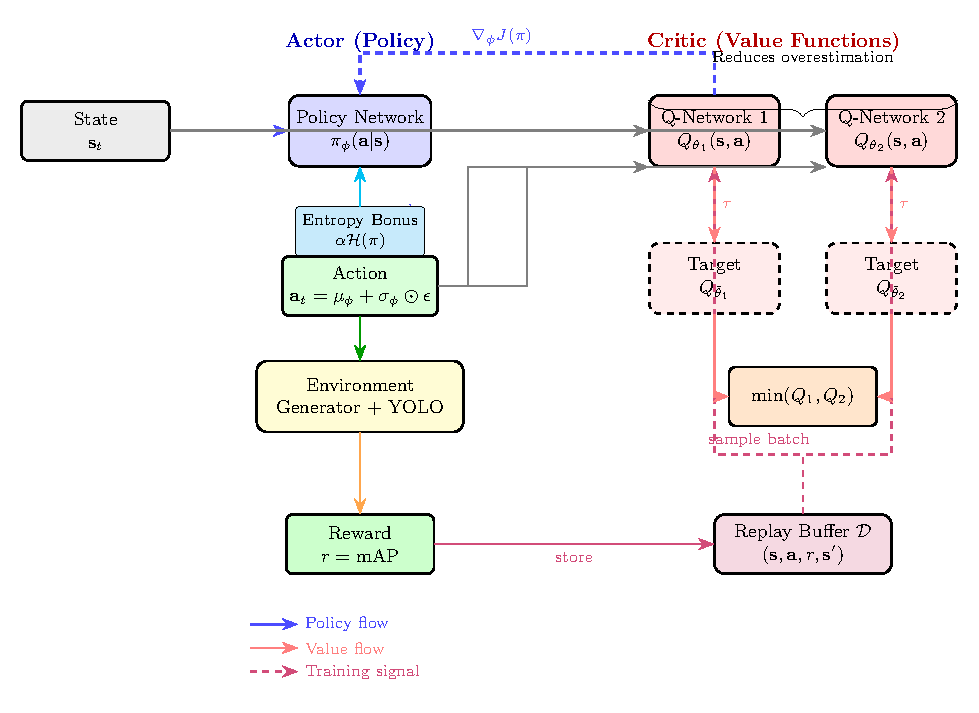
\includegraphics[width=0.95\textwidth]{figures/ch03_fig1_actor_critic.pdf}
\caption{Actor-critic architecture for generator parameter optimization. The actor network outputs parameter configurations as actions, which are evaluated through the generator and YOLO training pipeline. The twin critic networks estimate action values, with the minimum used for target computation to reduce overestimation. Soft updates transfer critic weights to target networks. The replay buffer stores transitions for off-policy learning. The entropy bonus encourages exploration and prevents premature policy collapse.}
\label{fig:actor_critic}
\end{figure}


\section{Convergence Analysis and Algorithm Selection Guidelines}
\label{sec:convergence}

The convergence properties of optimization algorithms provide theoretical guidance for algorithm selection, though practical performance depends on problem-specific factors that may not be captured by asymptotic analysis. This section summarizes convergence results and provides practical guidelines for selecting among the algorithms presented in this chapter.

\subsection{Convergence Rate Comparison}
\label{subsec:convergence_rates}

Table~\ref{tab:convergence} summarizes theoretical convergence rates for the major algorithm classes, expressed in terms of the number of function evaluations required to achieve $\epsilon$-optimal solutions.

\begin{table}[htbp]
\centering
\caption{Convergence Rates of Optimization Algorithms}
\label{tab:convergence}
\renewcommand{\arraystretch}{1.3}
\begin{tabular}{|p{2.5cm}|p{3.0cm}|p{3.0cm}|p{3.5cm}|}
\hline
\textbf{Algorithm} & \textbf{Rate} & \textbf{Assumptions} & \textbf{Notes} \\
\hline
GP-BO (EI) & $O\left(\frac{(\log n)^{d+1}}{n}\right)$ & Smooth objective, known kernel & Near-optimal for smooth functions \\
\hline
GP-BO (UCB) & $O\left(\sqrt{\frac{\gamma_n}{n}}\right)$ & Bounded RKHS norm & $\gamma_n$ is information gain \\
\hline
TPE & $O\left(\frac{1}{\sqrt{n}}\right)$ & Lipschitz objective & Dimension-independent rate \\
\hline
CMA-ES & $O\left(\frac{d}{n}\right)$ & Convex, quadratic & Linear in dimension \\
\hline
Random Search & $O\left(\frac{1}{n^{1/d}}\right)$ & Lipschitz objective & Exponential in dimension \\
\hline
Policy Gradient & $O\left(\frac{1}{\sqrt{n}}\right)$ & Smooth policy class & High variance constants \\
\hline
\end{tabular}
\end{table}

Gaussian process Bayesian optimization with Upper Confidence Bound achieves a regret bound of $O(\sqrt{\gamma_n / n})$, where $\gamma_n$ is the maximum information gain about the objective function from $n$ observations. For common kernels, $\gamma_n$ grows polylogarithmically in $n$, yielding near-optimal rates. The Expected Improvement acquisition function achieves similar rates under slightly different assumptions, with the constant factors depending on the problem-specific regularity of the objective.

Tree-Parzen Estimators achieve a dimension-independent convergence rate under Lipschitz assumptions, though the constant factors may depend exponentially on dimension in worst-case settings. The practical performance of TPE often exceeds what the worst-case analysis suggests, particularly for structured problems where only a subset of parameters significantly affects the objective.

Evolution strategies such as CMA-ES converge linearly for convex quadratic functions, with rates that scale favorably with dimension. For non-convex functions, the analysis is more complex, but empirical performance remains strong. The population-based nature of CMA-ES enables parallel evaluation, which can compensate for lower per-evaluation efficiency when parallel resources are available.

\subsection{Practical Algorithm Selection}
\label{subsec:practical_selection}

The choice of optimization algorithm for generator parameter optimization should be guided by the following considerations. First, the evaluation budget determines which algorithms are feasible. With fewer than 100 evaluations, Gaussian process Bayesian optimization with Expected Improvement provides the best expected performance, as the cubic scaling is not yet problematic and sample efficiency is paramount. With 100 to 1000 evaluations, TPE and BOHB become competitive, offering better scaling without substantial loss of efficiency. Beyond 1000 evaluations, evolutionary methods and reinforcement learning algorithms become viable, particularly when parallel evaluation is available.

Second, the parameter space structure influences algorithm suitability. Purely continuous spaces of moderate dimension favor Gaussian process methods. Mixed continuous-categorical spaces favor TPE and SMAC. Very high-dimensional spaces may require dimensionality reduction or local optimization methods such as TuRBO. Conditional parameter spaces require specialized handling available in TPE and SMAC but not standard Gaussian process implementations.

Third, the availability of multi-fidelity approximations changes the analysis. When cheap approximations to the objective are available, such as training with fewer epochs or smaller datasets, BOHB offers substantial acceleration by intelligently allocating resources across fidelity levels. Without multi-fidelity structure, BOHB reduces to standard TPE with the overhead of bracket management.

Fourth, the desire for schedule discovery rather than fixed configurations argues for Population-Based Training. When the optimal parameters vary over the course of YOLO training, PBT's online adaptation discovers effective schedules that fixed-configuration methods cannot find. This advantage is most relevant when the generator can be integrated into the training loop, producing data adaptively.

The algorithms presented in this chapter provide a comprehensive toolkit for generator parameter optimization. Bayesian optimization methods offer the best sample efficiency for expensive single-point evaluations. Population-Based Training enables schedule discovery when parameters should vary over training. Continuous control reinforcement learning methods become competitive when evaluation costs can be reduced or prior knowledge can be transferred. The practitioner should select among these approaches based on the specific characteristics of their optimization problem, guided by the analysis and comparisons provided in this chapter.


\section{Summary}
\label{sec:chapter_summary}

This chapter has provided a comprehensive treatment of reinforcement learning and related optimization algorithms for synthetic data generator parameter optimization. The key insights developed across the sections provide a foundation for practical algorithm deployment.

The fundamental limitation of traditional reinforcement learning for expensive black-box optimization stems from sample complexity requirements that exceed practical evaluation budgets by orders of magnitude. Bayesian optimization addresses this limitation through probabilistic surrogate modeling that enables intelligent exploration with limited evaluations. The Tree-Parzen Estimator provides a scalable alternative to Gaussian process models, handling high-dimensional and mixed parameter spaces while maintaining sample efficiency.

BOHB combines Bayesian optimization with multi-fidelity scheduling, exploiting the observation that performance rankings often stabilize before full evaluation completes. The integration of TPE sampling with successive halving achieves acceleration proportional to the correlation between low-fidelity and high-fidelity evaluations, with graceful degradation when such structure is absent.

Population-Based Training provides a complementary paradigm that discovers parameter schedules through online adaptation. Rather than searching for optimal fixed configurations, PBT maintains a population of agents that share information through exploitation and exploration operations. The resulting schedules often outperform fixed configurations, particularly for parameters whose optimal values change over the course of training.

Continuous control reinforcement learning methods including Soft Actor-Critic and Twin Delayed DDPG offer alternatives when evaluation costs can be reduced or when transfer learning from related tasks is possible. The maximum entropy framework underlying SAC provides theoretical grounding for exploration and robustness, with practical benefits for transfer and generalization.

The design of state and action representations influences optimization performance across all algorithm classes. Careful handling of continuous, discrete, and conditional parameters enables efficient search, while hierarchical decomposition reduces effective dimensionality. State representations that incorporate optimization history enable transfer of knowledge across the search trajectory.

Sample efficiency techniques including prioritized experience replay, transfer learning, and surrogate modeling maximize the information extracted from expensive evaluations. These techniques are essential for practical deployment in resource-constrained settings where each YOLO training run represents a substantial computational investment.

The convergence analysis and practical guidelines presented in this chapter provide a framework for algorithm selection based on problem characteristics. Budget constraints, parameter space structure, multi-fidelity availability, and schedule discovery requirements all influence the appropriate algorithm choice. The comprehensive treatment of leading algorithms equips practitioners to make informed decisions for their specific optimization challenges.

\end{chapter}
